\documentclass[../main/main.tex]{subfiles}
\begin{document}
\dominitoc
\faketableofcontents
\setcounter{chapter}{6}
\chapter{Modélisation de scène et extraction de sources}\label{ch:res}
\minitoc
\vspace{2cm}
Ce chapitre est consacré à la description de la dernière étape du pipeline \hypergal, la
modélisation de scène. Les chapitres précédents ont permis dans un
premier temps la
construction du cube intrinsèque de la galaxie hôte. Puis nous avons
procédé à sa projection dans
l'espace spectral de la SEDm à partir de la réponse impulsionnelle
spectrale de l'instrument. Enfin, nous avons également construit un modèle
de PSF robuste permettant la modélisation de sources ponctuelles.

Dans ce chapite, nous allons tout d'abord détailler le processus de
modélisation de scène, puis nous présenterons les résultats d'extraction des
différentes composantes qui la composent. Après avoir montré ces
résultats pour un cas idéal, nous montrerons quelques extractions de cas
plus complexes obtenus avec \hypergal.
\newpage

\section{Modélisation de scène}
% \label{sec:xxx}

\subsection{Présentation de la méthode}
%\label{sec:xxx}

La modélisation de scène implémentée dans \hypergal\ va globalement
suivre la méthode utilisée pour l'extraction de source ponctuelle,
présentée dans le chapitre précédent.

L'idée est de modéliser la scène pour $N$ méta-tranches couvrant un
domaine spectral pertinent de la SEDm. En effectuant un ajustement de la
scène pour chaque méta-tranche, nous obtiendrons un jeu de
$N$ paramètres. Puis, à l'instar de la méthode d'extraction de source
ponctuelle, nous procèderons à un ajustement de la chromaticité des
différentes composantes de la scène. Cela nous permettra de fixer tous
les paramètres de forme et de position. Enfin nous terminerons par un ajustement linéaire
des amplitudes pour toutes les tranches du cube de données.

Cette procédure nécessite dans un premier temps de projeter notre cube
intrinsèque dans l'espace de la SEDm. Nous rappelons qu'à l'issue de la
détermination de la réponse impulsionnelle spectrale (LSF), nous avons
déjà projeté notre cube intrinsèque dans l'espace spectral de la
SEDm. Il nous manque donc la projection dans l'espace spatiale.

\subsection{Projection du cube intrinsèque}
%\label{sec:xxx}

La projection du cube ne se fait pas en une opération, mais en projetant
successivement chaque tranche qui le compose.

Il nous faut pour cela prendre en compte la géométrie des spaxels des 2
cubes. Pour les traitements géométriques, nous utilisons le module
\pkg{shapely}\footnote{\url{https://github.com/shapely/shapely}} \citep{shapely2007}, qui
nous permet de reconstruire la grille avec les spaxels carrés du cube
intrinsèque, et celle avec les spaxels hexagonaux du cube de données
SEDm.

Avant de projeter le flux, nous adaptons l'échelle des pixels entre les
deux espaces. Nous savons que les pixels des images PS1 ont une taille
de $0\farcs25$ de côté. Afin de connaître précisément le facteur
d'échelle à appliquer, nous avons effectué une analyse spatiale sur des
observations de la SEDm avec un grand nombre ($>3$) de sources dans le
champ de vue. Par comparaison géométrique avec les images PS1 de la même
zone du ciel, analogue à une triangulation, nous avons déterminé un
rapport d'échelle de $2.230\pm0.003$ entre la taille des pixels de la
SEDm et des images PS1. Nous en avons déduit une taille effective des
spaxels hexagonaux de $0\farcs558$/spaxel. Il est important de
comprendre que cette adaptation d'échelle est purement numérique et ne correspond pas à
un ré-échantillonnage. La Figure~\ref{fig:scaleadapted} illustre
l'importance de prendre en compte cette différence de taille entre les spaxels.

\begin{figure}[ht]
  \centering
  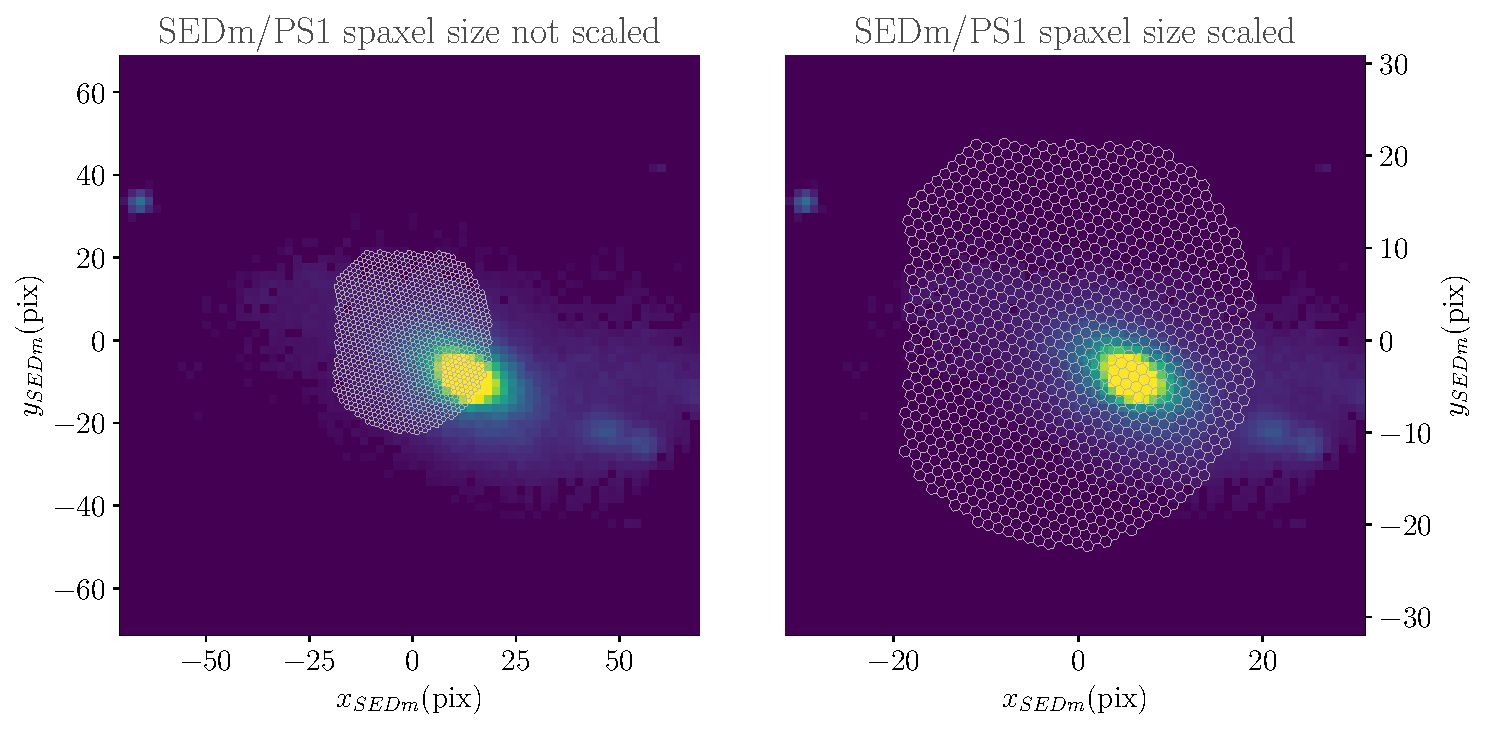
\includegraphics[width=0.9\textwidth]{../figures/07_scene/scaleadapted.png}
  \caption[Concordance des champs de vue PS1 et SEDm.]{Concordance des
    champs de vue PS1 et SEDm sur la supernova ZTF18accrorf en appliquant le rapport d'échelle entre
    la taille des pixels de chaque instrument. La grille hexagonale
    correspond au MLA de la SEDm, superposé sur une méta-tranche du cube
    intrinsèque empilé. La superposition illustrée ici aligne le centre
    du MLA et celui du cube.}
  \label{fig:scaleadapted}
\end{figure}

Avant de projeter le flux du cube intrinsèque, nous incluons un modèle de
correction du seeing. En effet, les images PS1 ayant un seeing plus
petit ($\sim1\farcs2$) que celui de la SEDm ($\sim2\arcsec$), nous
devons prendre en compte cette différence avant le ré-échantillonnage
spatial.

En toute rigueur, il faudrait entraîner un modèle de PSF relatif entre
PS1 et la SEDm. Dans ce travail, nous avons supposé que la correction du
seeing relatif pouvait être modélisée par une gaussienne 2D asymétrique
(présentant une potentielle ellipticité). Le seeing des images PS1 et
de la SEDm n'étant pas fixes, les paramètres de ce modèle seront libres
dans notre modélisation de scène.

Après la convolution de la tranche considérée du cube intrinsèque par ce
kernel gaussien, nous devons déterminer une position d'ancrage entre la
grille hexagonale et la tranche du cube à projeter.

Cette ancre de projection doit être une position du ciel dont nous
connaissons la localisation à la fois dans les images PS1, et dans le
MLA de la SEDm. Par défaut dans \hypergal, nous utilisons la position
de l'évènement transitoire détectée par la caméra ZTF, à partir de
laquelle nous avons récupéré les images PS1. La caméra de guidage de la
SEDm (la \textit{Rainbow Camera}) nous fournit également une position
approximative de l'objet détecté dans le MLA.

Nous alignons ainsi cette position du MLA avec le centre de la tranche
du cube considérée avant d'effectuer la projection du flux.

Pour procéder à la projection du flux dans l'espace spatial de la SEDm,
nous utilisons le module
\pkg{geopandas}\footnote{\url{https://geopandas.org/}}
\citep{kelsey_jordahl_2020_3946761}.
Cet outil nous permet de superposer les deux grilles de polygones
décrivant les géométries du cube intrinsèque et du MLA, puis de
déterminer les aires de chevauchement entre tous les pixels. 

Nous récupérons ainsi pour chaque pixel du MLA l'intégrale des flux
du cube qui le chevauchent, en pondérant
par l'aire de superposition. Cette aire de superposition est égale à $1$
lorsque qu'un pixel carré du cube est entièrement contenu dans un pixel
hexagonal du MLA.

Nous présentons dans la Figure~\ref{fig:projecthost} la projection d'une
méta-tranche du cube intrinsèque dans l'espace de la SEDm, convoluée par
une gaussienne 2D sans ellipticité d'écart type 1 pixel ($=0\farcs5$). L'ancrage est effectué à
partir de la position de la supernova ZTF18accrorf dans le MLA estimée
par la caméra de guidage. 

\begin{figure}[ht]
  \centering
  \includegraphics[width=0.9\textwidth]{../figures/07_scene/projecthost.png}
  \caption[Projection de la galaxie hôte dans le MLA.]{Projection de la
    galaxie hôte dans le MLA pour une méta-tranche du cube
    intrinsèque. Pour l'illustration de cet example, nous avons convolué la tranche par une
    gaussienne 2D sans ellipticité d'écart type 1 pixel. La croix rouge indique la position de la supernova
    ZTF18accrorf estimée par la \textit{Rainbow Camera} dans le MLA, qui
    sert d'ancrage à la projection d'un espace spatial à l'autre.}
  \label{fig:projecthost}
\end{figure}

Nous procédons ainsi à cette projection pour chaque méta-tranche du cube
spectral. Tout comme avec les étoiles standards, les 
cubes de données SEDm sont affectés par les effets d'ADR, et ainsi la position d'ancrage varie en fonction de la
longueur d'onde.

Ces paramètres ($x_{0}$, $y_{0}$) sont donc également des paramètres
libres de notre modélisation de scène, et la position renseignée par la
\textit{Rainbow Camera} fait office de condition initiale.

À ce stade de la modélisation, toutes les contributions relatives entre
PS1 et la SEDm ont été prises en compte.
Nous pouvons à présent compléter la scène avec les composantes de fond
et de source ponctuelle.

\subsection{Composantes de la scène}

\subsubsection{Composante du fond: ciel et artefacts}
% \label{ssec:xxx}

Le fond du ciel ayant été retiré dans les images PS1 \citep{Waters2020},
il nous faut modéliser cette composante. Pour les mêmes raisons évoquées
dans le chapitre~\ref{ch:irf} avec l'extraction des étoiles standards,
nous choisissons de modéliser le fond par un polynome de second degrée
tel que:

\begin{equation}
  \label{eq:backgroundcurved2}
  \text{Bkgd}(x,y) =
  \begin{pmatrix}
    b_{xx} &  &  &  &  & \\ 
     & b_{yy} &  &  &  \makebox(0,0){\text{\huge0}} & \\ 
     &  & b_{xy} &  & & \\
     &  &  & b_{x} &  & \\ 
     & \makebox(0,0){\text{\huge0}}  &  &  & b_{y} & \\ 
     &  &  &  &  & b_{0}\\
  \end{pmatrix}
  % 
  \begin{pmatrix}
    x^{2}\\
    y^{2}\\
    xy \\
    x \\
    y \\
    1 \\
  \end{pmatrix}
\end{equation}
avec $x$ et $y$ les coordonnées dans le MLA. La constante $b_{0}$ est
donc utilisée pour modéliser l'uniformité du ciel, tandis que les autres
paramètres sont là pour corriger les artefacts présents dans le cube de données.

\subsubsection{Composante de la supernova}
% \label{ssec:xxx}

L'autre composante de la scène n'est autre que la supernova, une source
ponctuelle entièrement caractérisée par la PSF de la SEDm. Nous
utilisons donc bien évidemment le profil radial contraint établit au
chapitre~\ref{ch:irf}:
\begin{equation}
  \label{eq:psfmodelconstraint}
  PSF(r; \alpha, \eta) = N\left[\eta\times\exp\left(- \frac{r}{2(\sigma_{0}+\sigma_{1}\times\alpha)^{2}}\right) +
    \left( 1+\left( \frac{r}{\alpha}\right)^{2}\right)^{-(\beta_{0}+\beta_{1}\times\alpha)} \right]
\end{equation}
avec $r$ le rayon elliptique du profil radial, et les $\sigma_{i}$ et
$\beta_{i}$ fixés par l'entraînement du modèle.

La position de la
supernova à modéliser dans le MLA est supposée confondu avec la position
d'ancrage utilisée lors de la projection du cube intrinsèque. Cette
approximation signifie que nous considérons la position de détection
dans le ciel par la caméra ZTF suffisament précise et ne nécessitant pas de
donner de liberté à la position relative entre la galaxie et l'objet
détecté.

\subsection{Ajustement de la scene 2D}
% \label{ssec:xxx}

Toutes les composantes de la scène ayant été décrites, nous pouvons
passer à l'ajustement de la scène 2D, en considérant les méta-tranches
indépendamment les unes des autres.

Nous avons choisi par défaut dans \hypergal\ de considérer 6
méta-tranches dans l'intervalle
spectral $\lambda\in$[$5000$,$8500$]\AA. Ce choix est motivé par la
précision spectrale de la calibration en flux de la
Figure~\ref{fig:allratio_std} du chapitre précédent. Bien que notre
modèle de fond ait été conçu pour prévenir de potentiels artefacts
strucutrés, ceux-ci deviennent trop intenses au delà de ce domaine
spectral. En se restreignant à cet intervalle, nous réduisons le risque
de valeurs d'ajustements aberrantes pouvant compliquer par la suite l'ajustement
chromatique. De plus, la majorité des supernovae observées par la
SEDm sont des SNIea ($\sim75\%$), dont leur magnitude diminue fortement
vers le rouge, notamment au delà
de $8000$-$8500$\AA. Le contraste entre une SNIa et sa galaxie hôte dans une
méta-tranche au delà de ces valeurs est donc fortement réduit, ce qui
permet difficilement la contrainte sur les paramètres de forme de la
PSF. La Figure~\ref{fig:artefactssedmcube} illustre bien le type
d'artefacts auxquels nous faisons référence, notamment sur les bords des
cubes dans le bleu, et des franges d'interférences intenses dans le rouge.

\begin{figure}[ht]
  \centering
  \includegraphics[width=0.6\textwidth]{../figures/07_scene/artefactssedmcube.pdf}
  \caption[Exemple d'artefacts dans les cubes de données SEDm.]{Exemple
    d'artefacts dans les cubes de données SEDm pour
    ZTF18accrorf. Nous montrons \emph{à gauche} toutes les tranches en dessous de
    $4800$\AA\ du cube de données empilées, et \emph{à droite}, toutes celles au dessus de
    $8700$\AA. Nous pouvons clairement voir dans le bleu la dégradation
    importante du signal, distordant complètement les objets dans le
    champ de vue, et également la présence d'artefacts de fond sur les
    bords du cube. Dans le rouge la forme des sources est également
    altérée, mais nous voyons surtout des franges d'interférences dans
    les données.}
  \label{fig:artefactssedmcube}
\end{figure}

Nous présentons dans la Table~\ref{tab:paramshypergal} la liste des
paramètres libres de la modélisation de scène pour une méta-tranche.
\begin{table}
  \scriptsize
  \centerfloat
  \setlength\tabcolsep{14pt}
  \renewcommand{\arraystretch}{1.5}
  \begin{threeparttable}
    \caption[Paramètres de modélisation de scène 2D avec \hypergal.]{Paramètres de modélisation de scène incluant toutes les
      composantes pour une méta-tranche dans \hypergal.}
    \label{tab:paramshypergal}
    \begin{tabular}{ccc}
      \toprule                               
      \textbf{Paramètre} &  & \textbf{Symbole} \\            
      \midrule
                         &\textbf{Géométrie}& \\
      \hline 
      Position d'ancrage  & & $x_{0}$, $y_{0}$\\
      
      \hline
      
                         &\textbf{Galaxie hôte}& \\
      
      \hline
      PSF relative SEDm/PS1 &  & $\sigma$ \\
      Ellipticité (PSF relative) &  & $\mathcal{A}_{G}$, $\mathcal{B}_{G}$\\
      Amplitude & & $G$\\
      
      \hline                               

                         &\textbf{Fond}& \\
      \hline
      
      Artefacts& & $b_{xx}$, $b_{yy}$, $b_{xy}$, $b_{x}$, $b_{y}$\\
      Ciel & & $b_{0}$\\
      
      \hline
                         &\textbf{Source ponctuelle (SN)}&\\
      
      \hline
      PSF SEDm  & & $\alpha$, $\eta$\\
      
      Ellipticité (PSF) &  & $\mathcal{A}$, $\mathcal{B}$\\
      Amplitude & & $I$ \\
      
      \bottomrule
    \end{tabular}
    \begin{tablenotes}[flushleft]
    \item \textbf{Note.} Les paramètres d'amplitudes et de fond sont
      des paramètres de nuisance dans la modélisation des méta-tranches. 
    \end{tablenotes}
  \end{threeparttable}
\end{table}

L'ajustement se fait par minimisation de $\chi^{2}$, défini comme:

\begin{equation}
  \label{eq:chi2hypergal}
  \chi^{2}=\sum\limits_{pixel}\left(\frac{(y_{p} - \widetilde{y}_{p})^{2}}{\sigma_{p}^{2}}\right)
\end{equation}
où $y_{p}$ et $\sigma_{p}$ sont respectivement le flux et la racine de
la variance dans un pixel $p$ de la méta-tranche du cube SEDm, et
$\widetilde{y}_{p}$ le flux modélisé dans ce même pixel.
Nous effectuons la minimisation avec le module
\pkg{iminuit}\footnote{\url{https://iminuit.readthedocs.io/en/stable/}} \citep{James:1975dr,iminuit}.

La procédure de construction de la scène pour une méta-tranche et pour
chaque pas de minimisation du $\chi^{2}$ se fait de la façon
suivante:

\begin{minipage}{\textwidth}%
  \begin{enumerate}[(a)]
    \itemsep=0em
  \item Convolution de la méta-tranche du cube intrinsèque par un kernel
    gaussien 2D asymétrique avec un paramètre d'amplitude;
  \item Projection dans l'espace spatiale de la SEDm suivant à partir de
    la position d'ancrage;
  \item Ajout du fond structuré (ciel + artefacts);
  \item Ajout de la source ponctuelle (PSF + amplitude);
  \item Détermination du $\chi^{2}$, puis réitération des étapes précédentes;
  \end{enumerate}
\end{minipage}\\

Nous présentons dans la Figure~\ref{fig:metaslicescene} l'ajustement des
$6$ méta-tranches par \hypergal\ pour ZTF18accrorf. Pour chaque longueur
d'onde, nous montrons la scène ajustée, la scène observée, et le résidu
avec le RMS spatial associé. Dans le cas de cette observation, notre RMS
spatial varie de $1.8\%$ à $3.9\%$. Nous pouvons également remarqué
l'augmentation de RMS pour la méta-tranche la plus \textit{bleue}
centrée sur $5285$\AA, probablement à cause d'un fond de plus en plus
structuré comme illustré dans la Figure~\ref{fig:artefactssedmcube}. La
méta-tranche la plus \textit{rouge} à $8200$\AA\ commence également à
présenter des artefacts structurés, vraisemblablement des franges de
Moiré (phénomène d'interférences).

\begin{figure}
  \centering
  \includegraphics[width=0.8\textwidth]{../figures/07_scene/fitted_metasliceZTF18accrorf_0.png}
  \includegraphics[width=0.8\textwidth]{../figures/07_scene/fitted_metasliceZTF18accrorf_1.png}
  \includegraphics[width=0.8\textwidth]{../figures/07_scene/fitted_metasliceZTF18accrorf_2.png}
  \includegraphics[width=0.8\textwidth]{../figures/07_scene/fitted_metasliceZTF18accrorf_3.png}
  \includegraphics[width=0.8\textwidth]{../figures/07_scene/fitted_metasliceZTF18accrorf_4.png}
  \includegraphics[width=0.8\textwidth]{../figures/07_scene/fitted_metasliceZTF18accrorf_5.png}
  \caption[Ajustement des méta-tranches pour la modélisation de scène de ZTF18accrorf.
  ]{Ajustement des méta-tranches pour la modélisation de scène de
    ZTF18accrorf. \emph{De haut en bas} sont représentées les
    méta-tranches modélisées du bleu vers le rouge. Pour chaque ligne
    \emph{de gauche à droite}: La méta-tranche modélisée par \hypergal,
    la méta-tranche du cube de données SEDm, et le résidu pondéré par le
  modèle. Nous indiquons pour chaque longueur d'onde le RMS spatial de
  l'ajustement, allant de $1.8\%$ à $3.9\%$. Les croix noires et rouges
  indiquent respectivement la position d'ancrage initiale (caméra de
  guidage), et la position ajustée par \hypergal.}
  \label{fig:metaslicescene}
\end{figure}

La Figure~\ref{fig:corrmatrixmetaslice} quant à elle présente la matrice
de corrélation entre les paramètres libres de la scène pour la
méta-tranche à $\lambda=6461$\AA.
\begin{figure}
  \centering
  \includegraphics[width=0.95\textwidth]{../figures/07_scene/heatmapcorrelation_metaslice.pdf}
  \caption[Matrice de corrélation des paramètres d'ajustement de scène
  pour une méta-tranche.]{Matrice de corrélation des paramètres
    d'ajustement de scène de ZTF18accrorf pour la méta-tranche à $\lambda=6461$\AA.}
  \label{fig:corrmatrixmetaslice}
\end{figure}

\subsection{Ajustement chromatique}
% \label{ssec:xxx}
L'ajustement de chaque méta-tranche nous donne ainsi un jeu de $N$
paramètres sur le domaine spectral [$5000$,$8000$]\AA. Nous modélisons
la chromaticité de la PSF de la source ponctuelle de la même manière
qu'avec les étoiles standards: une loi de puissance pour $\alpha$ (rayon
de la Moffat), et
une constante pour $\eta$ (poids gaussienne/Moffat), $\mathcal{A}$ et
$\mathcal{B}$ (ellipticité et orientation).

Nous utilisons également pour l'ellipticité et l'orientation de la PSF
relative (SEDm/PS1) une modélisation chromatique par une constante.

La chromaticité du rayon de la gaussienne de cette PSF relative est
modélisée par une loi de puissance, de la même façon que le paramètre de forme principal de la
source ponctuelle:
\begin{equation}
  \label{eq:sigmahostchrom}
  \sigma(\lambda)=\sigma_{ref}\left(\frac{\lambda}{\lambda_{ref}}\right)^{\rho_{g}}
\end{equation}


\begin{figure}
  \centering
  \includegraphics[width=0.7\textwidth]{../figures/07_scene/chromaticity_targetZTF18accrorf.pdf}
  \caption[Chromaticité des paramètres de forme de la PSF de la supernova ZTF18accrorf]{Ajustement de
    la chromaticité
    des paramètres de forme de la PSF pour la supernova ZTF18accrorf, à
    partir des 6 méta-tranches. \emph{À gauche} l'ajustement du paramètre $\alpha$ avec une
    loi de puissance. \emph{À droite} de haut en bas, l'ajustement par une
    constante de $\eta$ (poids entre la gaussienne et la Moffat) et des
    paramètres d'ellipticité ($\mathcal{A}$) et d'orientation ($\mathcal{B}$). }
  \label{fig:chromaticity_target}
\end{figure}


\section{Extraction des composantes}

\subsection{Outputs de controle du pipeline}
% \label{ssec:xxx}

\subsection{Extraction de la galaxie hôte}
% \label{ssec:xxx}

\subsection{Extraction de la Supernova}
% \label{ssec:xxx}

\section{Classification: \pkg{SNID}}
% \label{ssec:xxx}

\bibliographystyle{../main/aa_url2}
\bibliography{99_references}

\end{document}

%%% Local Variables:
%%% mode: latex
%%% TeX-master: t
%%% End:
